\section{Resolver el Juego Kuhn Poker}

Para resolver este juego se utilizó el procedimiento de Regret Matching con \textit{regret} incondicional, el cual es el más eficiente de los $3$ procedimientos descritos. Sin embargo, para poder aplicar este algoritmo es necesario llevar el juego a su forma normal, como se describe en la sección \ref{subsec:FN-FE}. Se realizó una corrida para obtener una estrategia hasta obtener un \textit{regret} menor que $10^{-5}$. El tiempo total fue de $3707.72$ segundos, y el número total de iteraciones fue de $535296954$. La Figura \ref{fig:regret-kuhn-poker} muestra el \textit{regret} con respecto al número de iteraciones. Se observa la convergencia a cero para ambos parámetros cuando el número de iteraciones tiende a infinito.

\begin{figure}[ht]
\caption{Gráfica del \textit{regret} con respecto al número de iteraciones del juego Kuhn Poker}
\label{fig:regret-kuhn-poker}
\centering
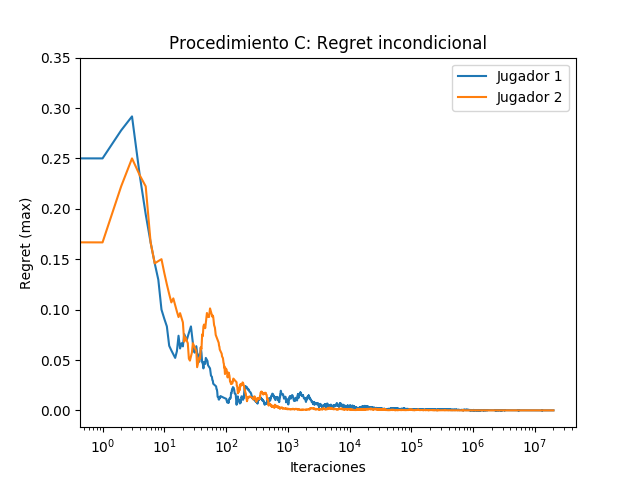
\includegraphics[width=1\textwidth]{graficas/kuhn/procedimiento-C.png}
\end{figure}

Para mostrar la estrategia obtenida, es necesario encontrar una estrategia de comportamiento equivalente a la estrategia mixta obtenida del algoritmo de \textit{Regret Matching}, como se describe en la sección \ref{subsec:EC-EM}. La Tabla \ref{tab:estrategia-kuhn-poker} muestra el equilibrio de Nash (parametrizado con la variable $\alpha$) y la estrategia obtenida del procedimiento. Se puede observar que la estrategia obtenida aproxima a un equilibrio de Nash con $\alpha \approx 0.249125$.

\begin{table}[ht]
    \centering
    \begin{tabular}{c|r r| r r}
        I & \multicolumn{2}{|c|}{Equilibrio de Nash} & \multicolumn{2}{|c}{Regret Matching} \\ \hline
         $1$ & $1-\alpha$ & $\alpha$ & $0.750875$ & $0.249125$ \\
         $2$ & $1$ & $0$ & $1$ & $0$ \\
         $3$ & $1$ & $0$ & $1$ & $0$ \\
         $4$ & $\frac{2}{3}$& $\frac{1}{3}$ & $0.666633$ & $0.333367$ \\
         $5$ & $0$ & $1$ & $0$ & $1$ \\
         $6$ & $1$ & $0$ & $1$ & $0$ \\
         $7$ & $0$ & $1$ & $0$ & $1$ \\
         $8$ & $\frac{2}{3}$ & $\frac{1}{3}$ & $0.666633$ & $0.333367$ \\
         $9$ & $\frac{2}{3} - \alpha$ & $\alpha + \frac{1}{3}$ & $0.417775$ & $0.582225$ \\
        $10$ & $1$ & $0$ & $1$ & $0$ \\
        $11$ & $1 - 3 \alpha$ & $3 \alpha$ & $0.253224$ & $0.746776$ \\
        $12$ & $0$ & $1$ & $0$ & $1$ \\ \hline
    \end{tabular}
    \caption{Equilibrio de Nash y estrategia obtenida para el juego de Kuhn Poker}
    \label{tab:estrategia-kuhn-poker}
\end{table}

Con la estrategia calculada se obtiene que peor caso para el primer jugador es igual a $v_1 = -0.0556501$ y el peor caso para el segundo jugador es $v_2 = 0.0555501$. Estos valores están bastantes cercas a la ganancia esperada cuando se utiliza el equilibrio de Nash, que es $-1/18$ y $1/18$, respectivamente. Se puede notar que la diferencia entre la ganancia esperada utilizando un equilibrio de Nash y la obtenida con las ganancias utilizadas es no mayor a $10 ^ {-4}$.
